\documentclass[a4paper,12pt]{report}
%\usepackage[acronym, labelref, glossaries, index, debug]{CEFET}
\usepackage[acronym, labelref]{CEFET}

\ExecuteBibliographyOptions{maxbibnames=99} %Substitui o et al e exibe todos os autores nas Referências

\addbibresource{Referencias.bib}

\title{TÍTULO DO TRABALHO:}

\subtitle{subtítulo do trabalho (se houver)}

\author{Nome do Autor}  

\date{ANO}

\location{Betim}

\advisor{\textbf{Orientador:} Título Nome}

\coadvisor{\textbf{Coorientador:} Título Nome (se houver)}

\committeeone{Prof. Título Nome - IFMG}
\committeetwo{Prof. Título Nome - IFMG}
\committeethree{Prof. Titulo Nome - IFMG}
\committeedate{ dia / mês / ano}

\institution{
  Instituto Federal de Educação Ciência e Tecnologia de Minas Gerais - \textit{Campus} Betim
  \\
  Engenharia Mecânica
}

\preamble{Trabalho de Conclusão de Curso apresentado à banca examinadora do curso de Engenharia Mecânica do Instituto Federal de Educação, Ciência e Tecnologia de Minas Gerais - \textit{Campus} Betim, como parte dos requisitos para obtenção do título de Bacharel em Engenharia Mecânica.}
%\newglossaryentry{latex}
{
    name=latex,
    description={Is a markup language specially suited
            for scientific documents}
}

\newglossaryentry{maths}
{
    name=mathematics,
    description={Mathematics is what mathematicians do}
}

%%%%%%%%%%%%%%%%%%%%%%%%%%%%%%%%%%%%%%%%%%%%%%%%%%%%%%
% Se gostou desse template, deixe sua estrela no GitHub:
% https://github.com/lucasmsoares96/Template-Monografia-CEFET-MG
%%%%%%%%%%%%%%%%%%%%%%%%%%%%%%%%%%%%%%%%%%%%%%%%%%%%%%

%%%%%%%%%%%%%%%%%%%%%%%%%%%%%%%%%%%%%%%%%%%%%%%%%%%%%%
% Adaptado para o padrão IFMG Betim - 08/2025
%%%%%%%%%%%%%%%%%%%%%%%%%%%%%%%%%%%%%%%%%%%%%%%%%%%%%%

\usepackage{lipsum}    % gera texto aleatório (remover)
\usepackage[justification=centering]{caption} %centraliza o título das figuras
\usepackage{titlesec}
\usepackage{array}
\usepackage{pdfpages}

\newcolumntype{P}[1]{>{\centering\arraybackslash}p{#1}} %novo comando de coluna P, que permite definir largura e centraliza os textos

\begin{document}
\maketitle % Capa                           (obrigatório)
% Lombada                                   (opcional)
\frenchspacing

\pretextual
\makecover % folha de rosto                 (obrigatório)
%\chapter*{Errata}

FERRIGNO, C. R. A. \textbf{Tratamento de neoplasias ósseas apendiculares com
    reimplantação de enxerto ósseo autólogo autoclavado associado ao plasma
    rico em plaquetas}: estudo crítico na cirurgia de preservação de membro em
cães. 2011. 128 f. Tese (Livre-Docência) - Faculdade de Medicina Veterinária e
Zootecnia, Universidade de São Paulo, São Paulo, 2011.

\begin{table}[htb]
    \center
    \footnotesize
    \begin{tabular}{|p{1.4cm}|p{1cm}|p{3cm}|p{3cm}|}
        \hline
        \textbf{Folha} & \textbf{Linha} & \textbf{Onde se lê} & \textbf{Leia-se} \\
        \hline
        1              & 10             & auto-conclavo       & autoconclavo     \\
        \hline
    \end{tabular}
\end{table}%          (opcional)
%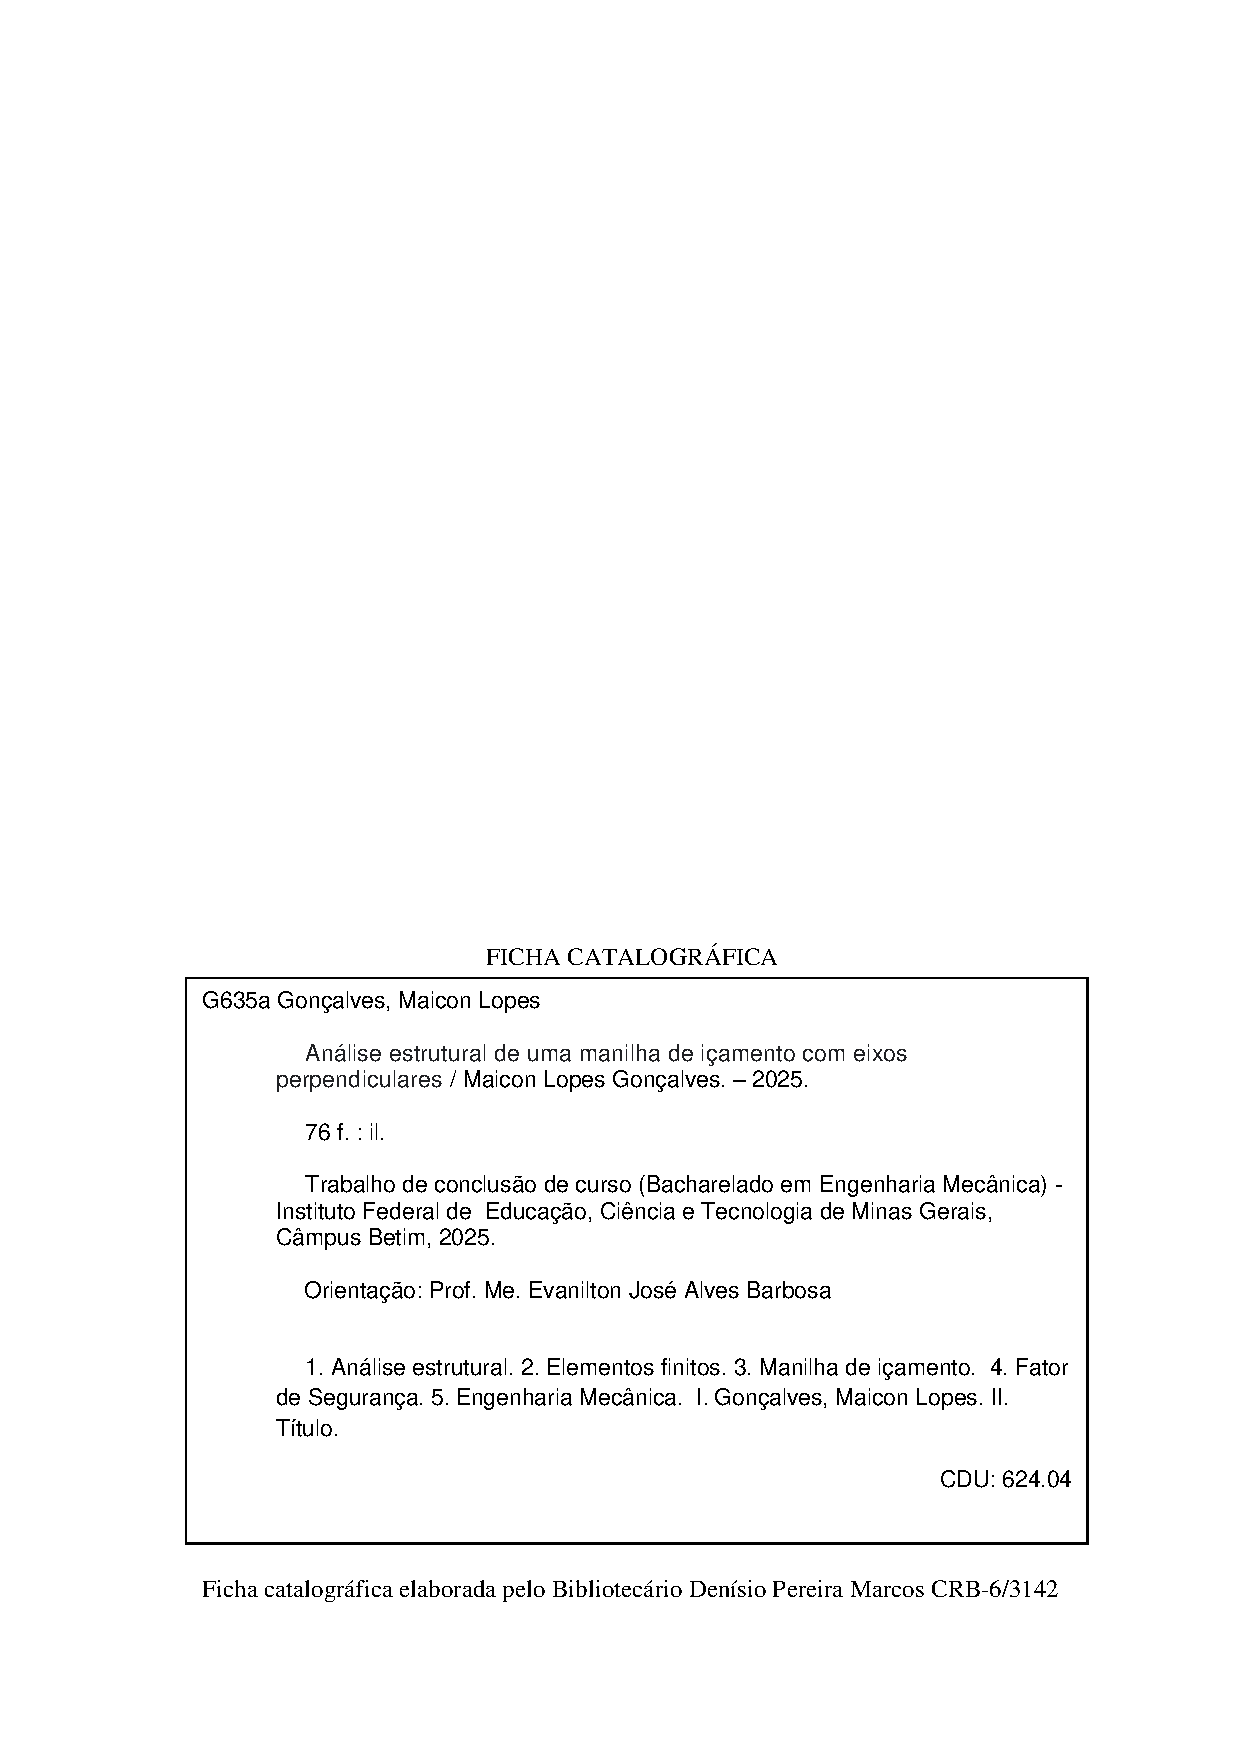
\includepdf{ficha_catalografica.pdf}%      (obrigatório) fornecido pela biblioteca
%
\includepdf{folha_aprovacao_assinada.pdf}% (obrigatório) 
\dedication{Dedico este trabalho a .}%      (opcional)
\chapter*{Agradecimentos}

Agradeço ao Instituto Federal de Educação, Ciência e Tecnologia de Minas Gerais - Campus Betim .
%   (opcional)
\epigraph{É perigoso, Frodo... sair porta afora, você pisa na estrada, e se não controlar os pés, não se sabe até onde pode ser levado.}{— J.R.R. Tolkien, O Senhor dos Anéis}

%\textit{Porque toda jornada começa com um passo — e, às vezes, esse passo nos leva além de tudo que sonhamos um dia.}%         (opcional)
\begin{abstract}
   Este trabalho tem como objetivo .
    \\ \\
    \textbf{Palavras-chave:} Manilha de Içamento; Método dos Elementos Finitos; ANSYS Workbench; Fator de Segurança; AISI 4340.

\end{abstract} %          (obrigatório)
\begin{otherlanguage}{english}
    \begin{abstract}
        This work presents .
        \\ \\
        \textbf{Keywords:} Lifting Shackle; Finite Element Method; ANSYS Workbench; Safety Factor; AISI 4340.
    \end{abstract}
\end{otherlanguage} %        (obrigatório)
\listoffigures %                            (opcional)
\listoftables  %                            (opcional)
\chapter*{Lista de Abreviaturas e Siglas}
\begin{acronym}[xxxxxxxxx]
  
  \item[IFMG] Instituto Federal de Minas Gerais
  \item[CAD] Computer Aided Design
  \item[CAE] Computer Aided Engineering

\end{acronym} %          (opcional)
\chapter*{Lista de Símbolos}
\begin{acronym}[xxxxxxxxx]
    
  \item[$ \sigma  $] Tensão normal
  \item[$ \sigma_{u}  $] Limite de resistência
  \item[$ \sigma_{e}  $] Limite de escoamento


  \item[$\leq$] Menor ou igual
\end{acronym} %        (opcional)
\tableofcontents %                          (obrigatório)

\setcounter{page}{14} % Inserir aqui o número de páginas antes da introdução menos a capa. Ex. se quiser que a introdução seja pg. 15, coloque o valor de 14.
\textual
\chapter{Introdução} \label{Introducao}



Dentro deste universo, a engenharia de componentes é fundamental. Conforme os princípios de Projeto de Máquinas detalhados por \textcite{Norton2013}, todo sistema mecânico deve ser analisado sob a ótica de suas cargas, tensões e modos de falha potenciais. Um acessório de içamento, como a manilha, embora aparentemente simples, é um componente submetido a complexos estados de tensão. Fenômenos como a concentração de tensão em seus raios de curvatura e furos, e o risco de falha por fadiga após ciclos repetidos de carregamento, são fatores críticos que governam sua vida útil e segurança. \textcite{Norton2013} enfatiza que a aplicação de adequados fatores de segurança no projeto não é uma mera formalidade, mas uma necessidade para mitigar os riscos associados a incertezas nas cargas e nas propriedades do material. Ignorar esses princípios de engenharia na seleção ou no uso de uma manilha é negligenciar a base científica que garante a segurança da operação.

\begin{figure}[!htb]
   \centering
    \caption{Variedade de montagens para içamento e movimentação de cargas.}
    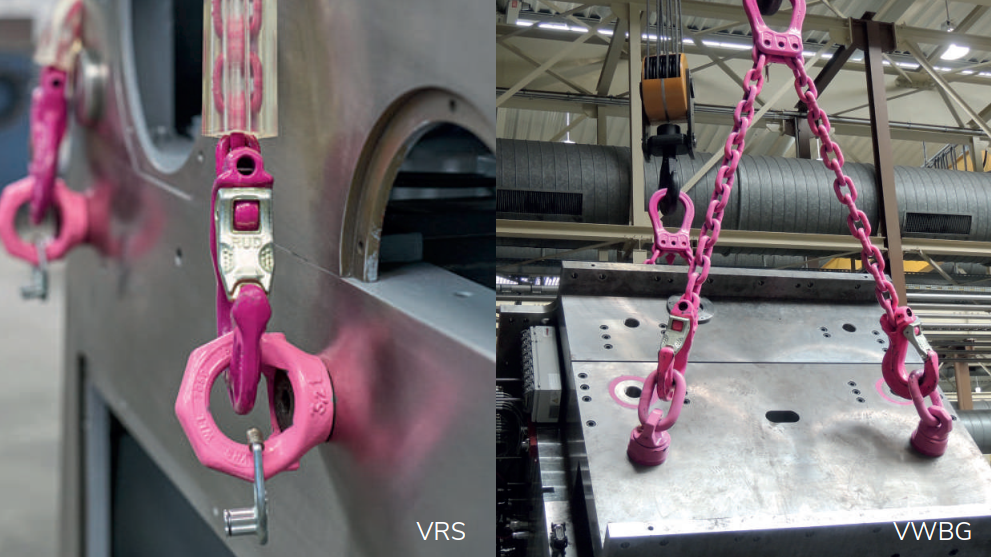
\includegraphics[width=1.0\linewidth]{Figuras/icamentoexemplos.png}\\    \hspace{1.5cm}\raggedright \fontsize{10}{12}\selectfont{Fonte: \textcite{RUD}.}
    \label{rudexemplos}
\end{figure}

A complexidade da seleção se aprofunda ao se consultar o portfólio de fabricantes especializados. O catálogo da \textcite{Crosby}, bem como a  \ref{rudexemplos}, que mostra montagens possíveis com produtos da RUD, referências no setor, ilustram que não existe uma solução única. A escolha deve ser criteriosa, distinguindo, por exemplo, entre manilhas tipo âncora (bow shackles), que são mais adequadas para cargas que vêm de múltiplos ângulos, e manilhas tipo reta (dee shackles), ideais para içamentos em linha. Adicionalmente, a seleção do sistema de travamento do pino é crucial: os modelos com pino roscado (screw pin) são práticos para montagens temporárias, enquanto os modelos com pino, porca e contrapino (bolt, nut, and cotter pin) são mandatórios para instalações de longo prazo ou onde há risco de vibração que poderia soltar o pino.



\section{Justificativa}

A utilização da análise de elementos finitos é uma excelente ferramenta para .

\section{Objetivos}

\subsection{Objetivo geral}

O objetivo deste trabalho é .  


\subsection{Objetivos específicos}
\begin{enumerate}

    \item Otimizar a .

    \item Definir .

    \item Definir .
    
\end{enumerate}
\chapter{Fundamentação teórica} \label{RevisaoBibliografica}

Este capítulo apresenta os fundamentos teóricos necessários .

\subsection{Tensão e Deformação}

Quando uma carga externa age sobre uma área seccionada de um corpo como na  \ref{pontoesp}, como resultado, aparecem forças internas agindo sobre essa mesma seção. Esse fenômeno é denominado tensão, que representa o quociente de uma força sobre uma área. Quando a força agir sobre a área perpendicularmente, tem-se a tensão normal \(\sigma \). Porém, quando a força agir tangencialmente à área, será denominada como tensão de cisalhamento \(\tau \), \cite{Hibbeler2009}.

\begin{figure}[!htb]
   \centering
     \caption{Cargas sobre um ponto.}
    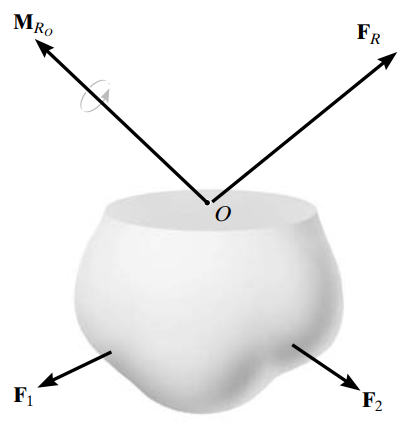
\includegraphics[width=0.3\linewidth]{Figuras/pontoespecifico.png}\\
    \hspace{1.5cm}\raggedright \fontsize{10}{12}\selectfont{Fonte: \textcite{Hibbeler2009}.}
    \label{pontoesp}
\end{figure}

Segundo \textcite{Hibbeler2009}, para um elemento de área infinitesimal \(\Delta \)A, a tensão normal \( \sigma_z \) se dará por um limite da razão da força \( F_z \) com a sua área tendendo a zero, como na equação \ref{eq1}:

\begin{equation}
\label{eq1}
\sigma_z =  \lim_{\Delta A\to0} \frac{\Delta F_z}{\Delta A} 
\end{equation}
\bigskip

Se essa força tracionar o elemento \(\Delta \)A, será denominada tensão de tração, ao passo que se comprimir o elemento, receberá o nome de tensão de compressão.
Para a tensão de cisalhamento (\(\tau \)) ocorre o mesmo fenômeno, dando origem a 2 componentes que agem tangencialmente à área infinitesimal \(\Delta \)A, sendo estes perpendiculares entre si, conforme as equações \ref{eq2a} e \ref{eq2b} \cite{Hibbeler2009}:

\begin{equation}
\label{eq2a}
\tau_{zx} =  \lim_{\Delta A\to0} \frac{\Delta F_x}{\Delta A}
\end{equation}
\bigskip

\begin{equation}
\label{eq2b}
\tau_{zy} =  \lim_{\Delta A\to0} \frac{\Delta F_y}{\Delta A}
\end{equation}
\bigskip


\chapter{Metodologia} \label{metodologia}

Este trabalho utilizou uma metodologia .

\section{Definição do Componente}

Dentro do campo de içamento 

\begin{figure}[!htb]
   \centering
     \caption{Componentes da manilha.}
    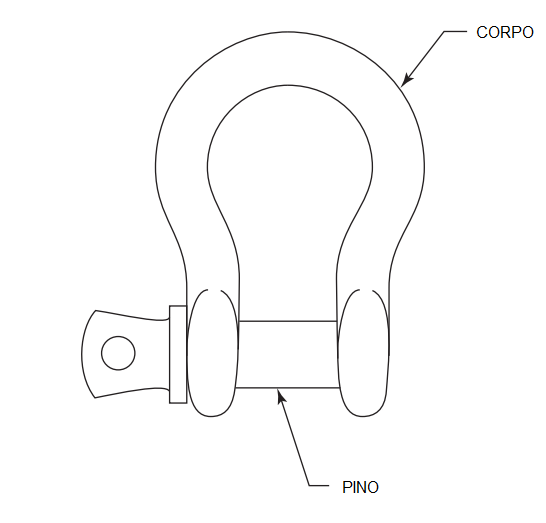
\includegraphics[width=0.45\linewidth]{Figuras/manilhacomponentes.png}\\
    \hspace{1.5cm}\raggedright \fontsize{10}{12}\selectfont{Fonte: Adaptado de \textcite{ASMEB3026}.}
    \label{manilhacomponentes}
\end{figure}

Manilhas comerciais possuem um formato típico, basicamente composto por um corpo em formato de arco e um pino de travamento, conforme  \ref{manilhacomponentes}. Existem muitas combinações possíveis para a montagem de manilhas em um conjunto de içamento e movimentação, entre essas combinações estão as montagens que se utilizam de múltiplas manilhas acopladas, como exemplificado na  \ref{manilhacombinacoes}. Visando essas combinações, a proposta deste trabalho é reproduzir essa combinação corpo-corpo em uma geometria única, de modo a verificar seu comportamento diante das solicitações de trabalho esperadas para o componente.

\begin{figure}[!htb]
   \centering
     \caption{Combinações de manilhas.}
    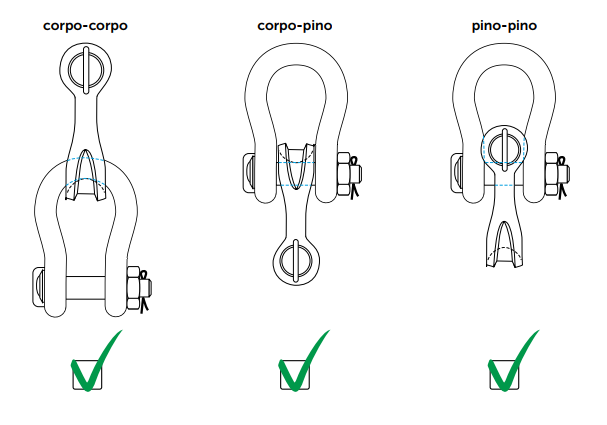
\includegraphics[width=0.65\linewidth]{Figuras/manilhacombinacoes.png}\\
    \hspace{1.5cm}\raggedright \fontsize{10}{12}\selectfont{Fonte: \textcite{GreenPin}.}
    \label{manilhacombinacoes}
\end{figure}

Como referência, foi utilizado a Super\textsuperscript{\textregistered}\hspace{0.1em} Manilha Curva SC, da Green Pin\textsuperscript{\textregistered}\hspace{0.1em}, padrão de excelência na fabricação e comercialização de manilhas no mercado internacional, conforme anexo A. Com corpo e pino em aço liga, grau 8, temperado e revenido.

Para requisitos iniciais, foram estabelecidos os parâmetros para verificação da geometria inicial conforme a  \ref{parametrosinicicais}. Como material do componente, foi escolhido o aço AISI 4340, com as propriedades mecânicas do componente tratado termicamente por têmpera e revenimento.

\begin{table}[!ht]
\centering
\caption{Parâmetros iniciais.}
\label{parametrosinicicais}
\begin{tabular}{ P{3cm} | P{3cm} | P{3cm} | P{3cm} } 
\hline
\textbf{Carregamento de Trabalho (kN)} & \textbf{Massa do Componente (kg) } & \textbf{Fator de segurança - FS} & \textbf{Diâmetro do Pino (mm)} \\ \hline
 10 & 1,0 & 5:1 & 19 \\ 
\hline
\end{tabular} \\
\smallskip
\hspace{1.5cm}\raggedright \fontsize{10}{12}\selectfont{Fonte: Elaborado pelo autor, 2025.}
\end{table}

\chapter{Resultados} \label{resultado}

Neste capítulo são apresentados os resultados obtidos .

\section{Carga de Tração}

Utilizando de exemplo a manilha da Green Pin que possui WLL de 49 kN (5 toneladas), conforme anexo A e levando em consideração que o componente se equipara à utilização de 2 manilhas comerciais, temos o comparativo conforme  \ref{comparativo}. Indicando que o WLL encontrado é coerente.

\begin{table}[!ht]
\centering
\caption{Comparativo da relação WLL x peso do componente.}
\label{comparativo}
\begin{tabular}{ P{2.5cm} | P{3cm} | P{2.5cm} | P{2.5cm} | P{3cm} } 
\hline
\textbf{Componente} & \textbf{WLL (kN)} & \textbf{Peso por unidade (kg) } & \textbf{Peso do conjunto (kg) } & \textbf{Relação kN/kg} \\ \hline
 Green Pin & 49,0 & 0,63 & 1,26 & 38,88\\ 
\hline
 Proposta & 42,5 & 1,07 & 1,07 & 39,71\\ 
\hline
\end{tabular} \\
\smallskip
\hspace{1.5cm}\raggedright \fontsize{10}{12}\selectfont{Fonte: Elaborado pelo autor, 2025.}
\end{table}

As maiores tensões equivalentes aparecem próximo às áreas de contato, com a tensão máxima equivalente aparecendo na face de contato do carregamento no furo superior, como mostra a  \ref{finalequivalente2}, bem como os fatores de segurança associados, indicados na  \ref{fatorsegurancafinal}.



\begin{figure}[!htb]
   \centering
     \caption{Fator de segurança na geometria final.}
    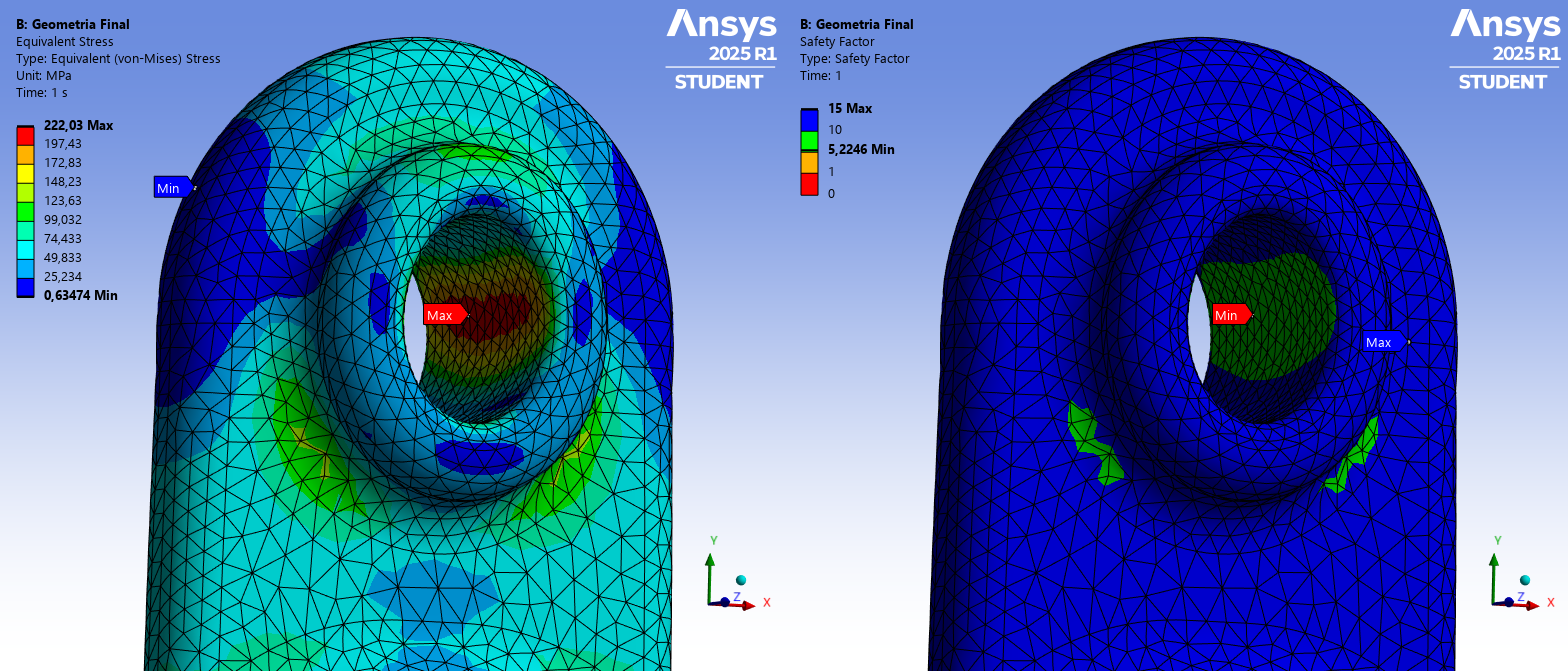
\includegraphics[width=1.0\linewidth, trim=0 0 0 0, clip]{Figuras/geometria final tensao equivalente 6.png}\\
    \hspace{1.5cm}\raggedright \fontsize{10}{12}\selectfont{Fonte: Elaborado pelo autor, 2025.}
    \label{fatorsegurancafinal}
\end{figure}

A título de comparação, a carga de trabalho de 42,5 kN foi aplicada na geometria inicial. Os resultados mostram uma tensão equivalente de Von Misses de 405,04 MPa e um fator de segurança mínimo de 2,86:1, indicando uma perda de 46 \% de capacidade para uma mesma carga de trabalho, como mostra a  \ref{fatorsegurancainicial}.

\begin{figure}[!htb]
   \centering
     \caption{Fator de segurança na geometria inicial.}
    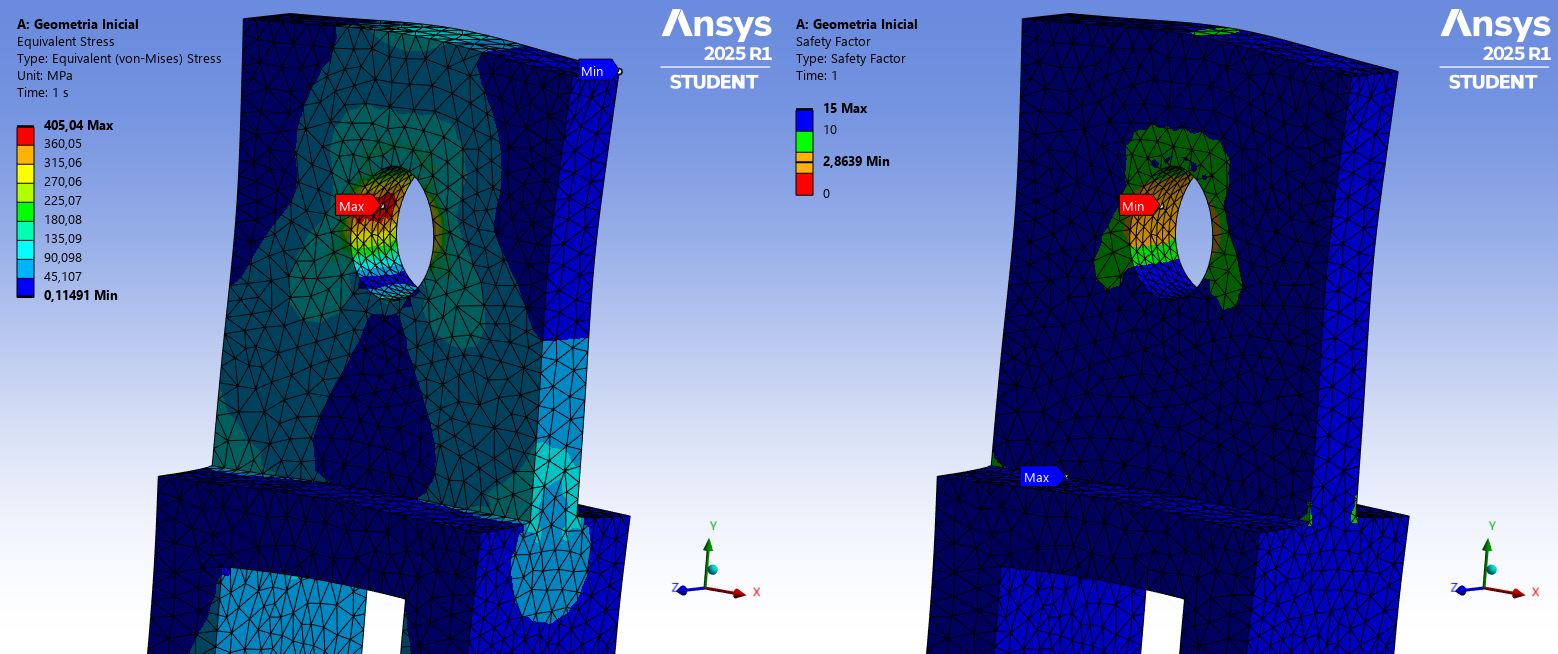
\includegraphics[width=1.0\linewidth, trim=0 0 0 0, clip]{Figuras/geometria inicial tensao equivalente 5.png}\\
    \hspace{1.5cm}\raggedright \fontsize{10}{12}\selectfont{Fonte: Elaborado pelo autor, 2025.}
    \label{fatorsegurancainicial}
\end{figure}



%\chapter{Considerações Finais} \label{consideracoes}

%%====== Section ========%
\chapter{Conclusão}\label{conclusao}

O presente trabalho teve como objetivo principal 
\chapter{Sugestões de trabalhos futuros}\label{Sugestões de trabalhos futuros}

\begin{itemize}

\item Levantamento de Custos: Propõe-se uma análise econômica completa do processo de forjamento, calculando todos os custos envolvidos - desde a matéria-prima e a fabricação das matrizes até as operações e tratamentos posteriores - para determinar o custo final por peça e confirmar a viabilidade financeira do projeto.
\item Simulação de Forjabilidade: Sugere-se o uso de simulação computacional para analisar o processo de forjamento, a fim de prever o fluxo do material, evitar defeitos, otimizar parâmetros e garantir que o componente final atinja as propriedades mecânicas e a integridade estrutural desejadas.
\item Análise Topológica: Recomenda-se a aplicação da otimização topológica para redesenhar o componente, buscando reduzir seu peso ao máximo sem comprometer a capacidade de carga (WLL). Este método utiliza algoritmo para encontrar a distribuição de material mais eficiente, gerando um design mais leve.

\end{itemize}

\postextual
\clearpage\pagestyle{empty}
\printbibliography %                 (obrigatório)
% \printglossaries %                   (opcional)
\clearpage\pagestyle{plain}

%-------------------------------------------------------------
%---------------------- Apêndices ----------------------------
%-------------------------------------------------------------
%Note que os Apêndices são dedicados aos textos ou \textbf{documentação elaborados pelo próprio autor} que complemente  a  argumentação  textual  (códigos,  reportagens,  relatórios  etc.).

\titlespacing*{\chapter}{0pt}{-10pt}{-2cm} 
\captionsetup[figure]{list=no} % Remove as figuras da lista
%\captionsetup[table]{list=no} % Remove as tabelas da lista

%\partapendices  % Indica o início dos Apendices

\chapter*{Apêndice A - Propriedades Mecânicas do AISI/SAE 4340}
\label{apendiceA}

\begin{figure}[h]
   \centering
    \caption{Propriedades do material no ANSYS Mechanical.}
    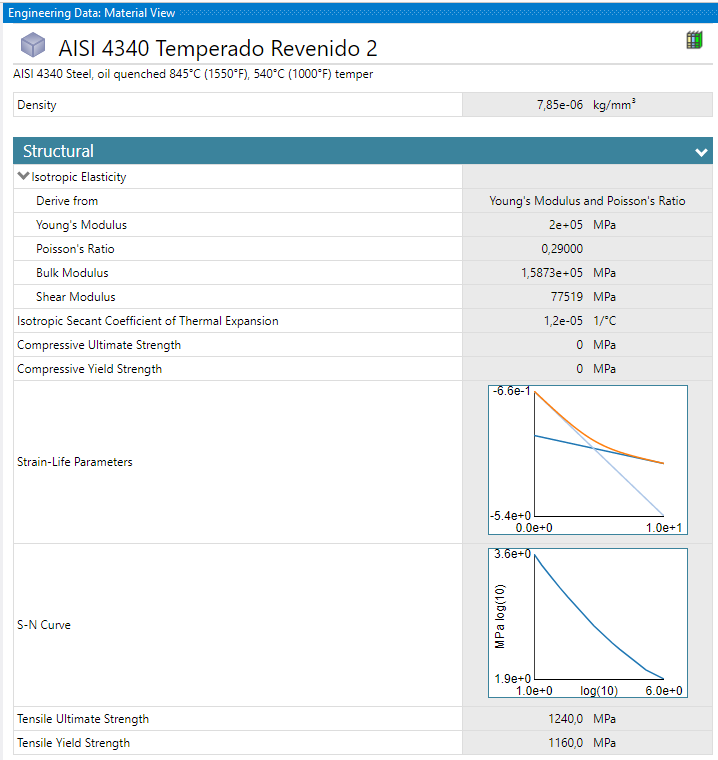
\includegraphics[width=1.0\linewidth, trim = 0 0 0 0, clip]{Figuras/4340Ansys2.png}\\
    \hspace{1.5cm}\raggedright \fontsize{10}{12}\selectfont{Fonte: Elaborado pelo autor, 2025.}
    \label{4340Ansys}
\end{figure}



 % (opcional)
\captionsetup[figure]{list=no} % Remove as figuras da lista
%\captionsetup[table]{list=no} % Remove as tabelas da lista


\chapter*{ANEXO A - Catálogo Manilha Green Pin.}
\label{anexoA}
\begin{figure}[!htb]
   \centering
    \caption{Manilha comercial.}
    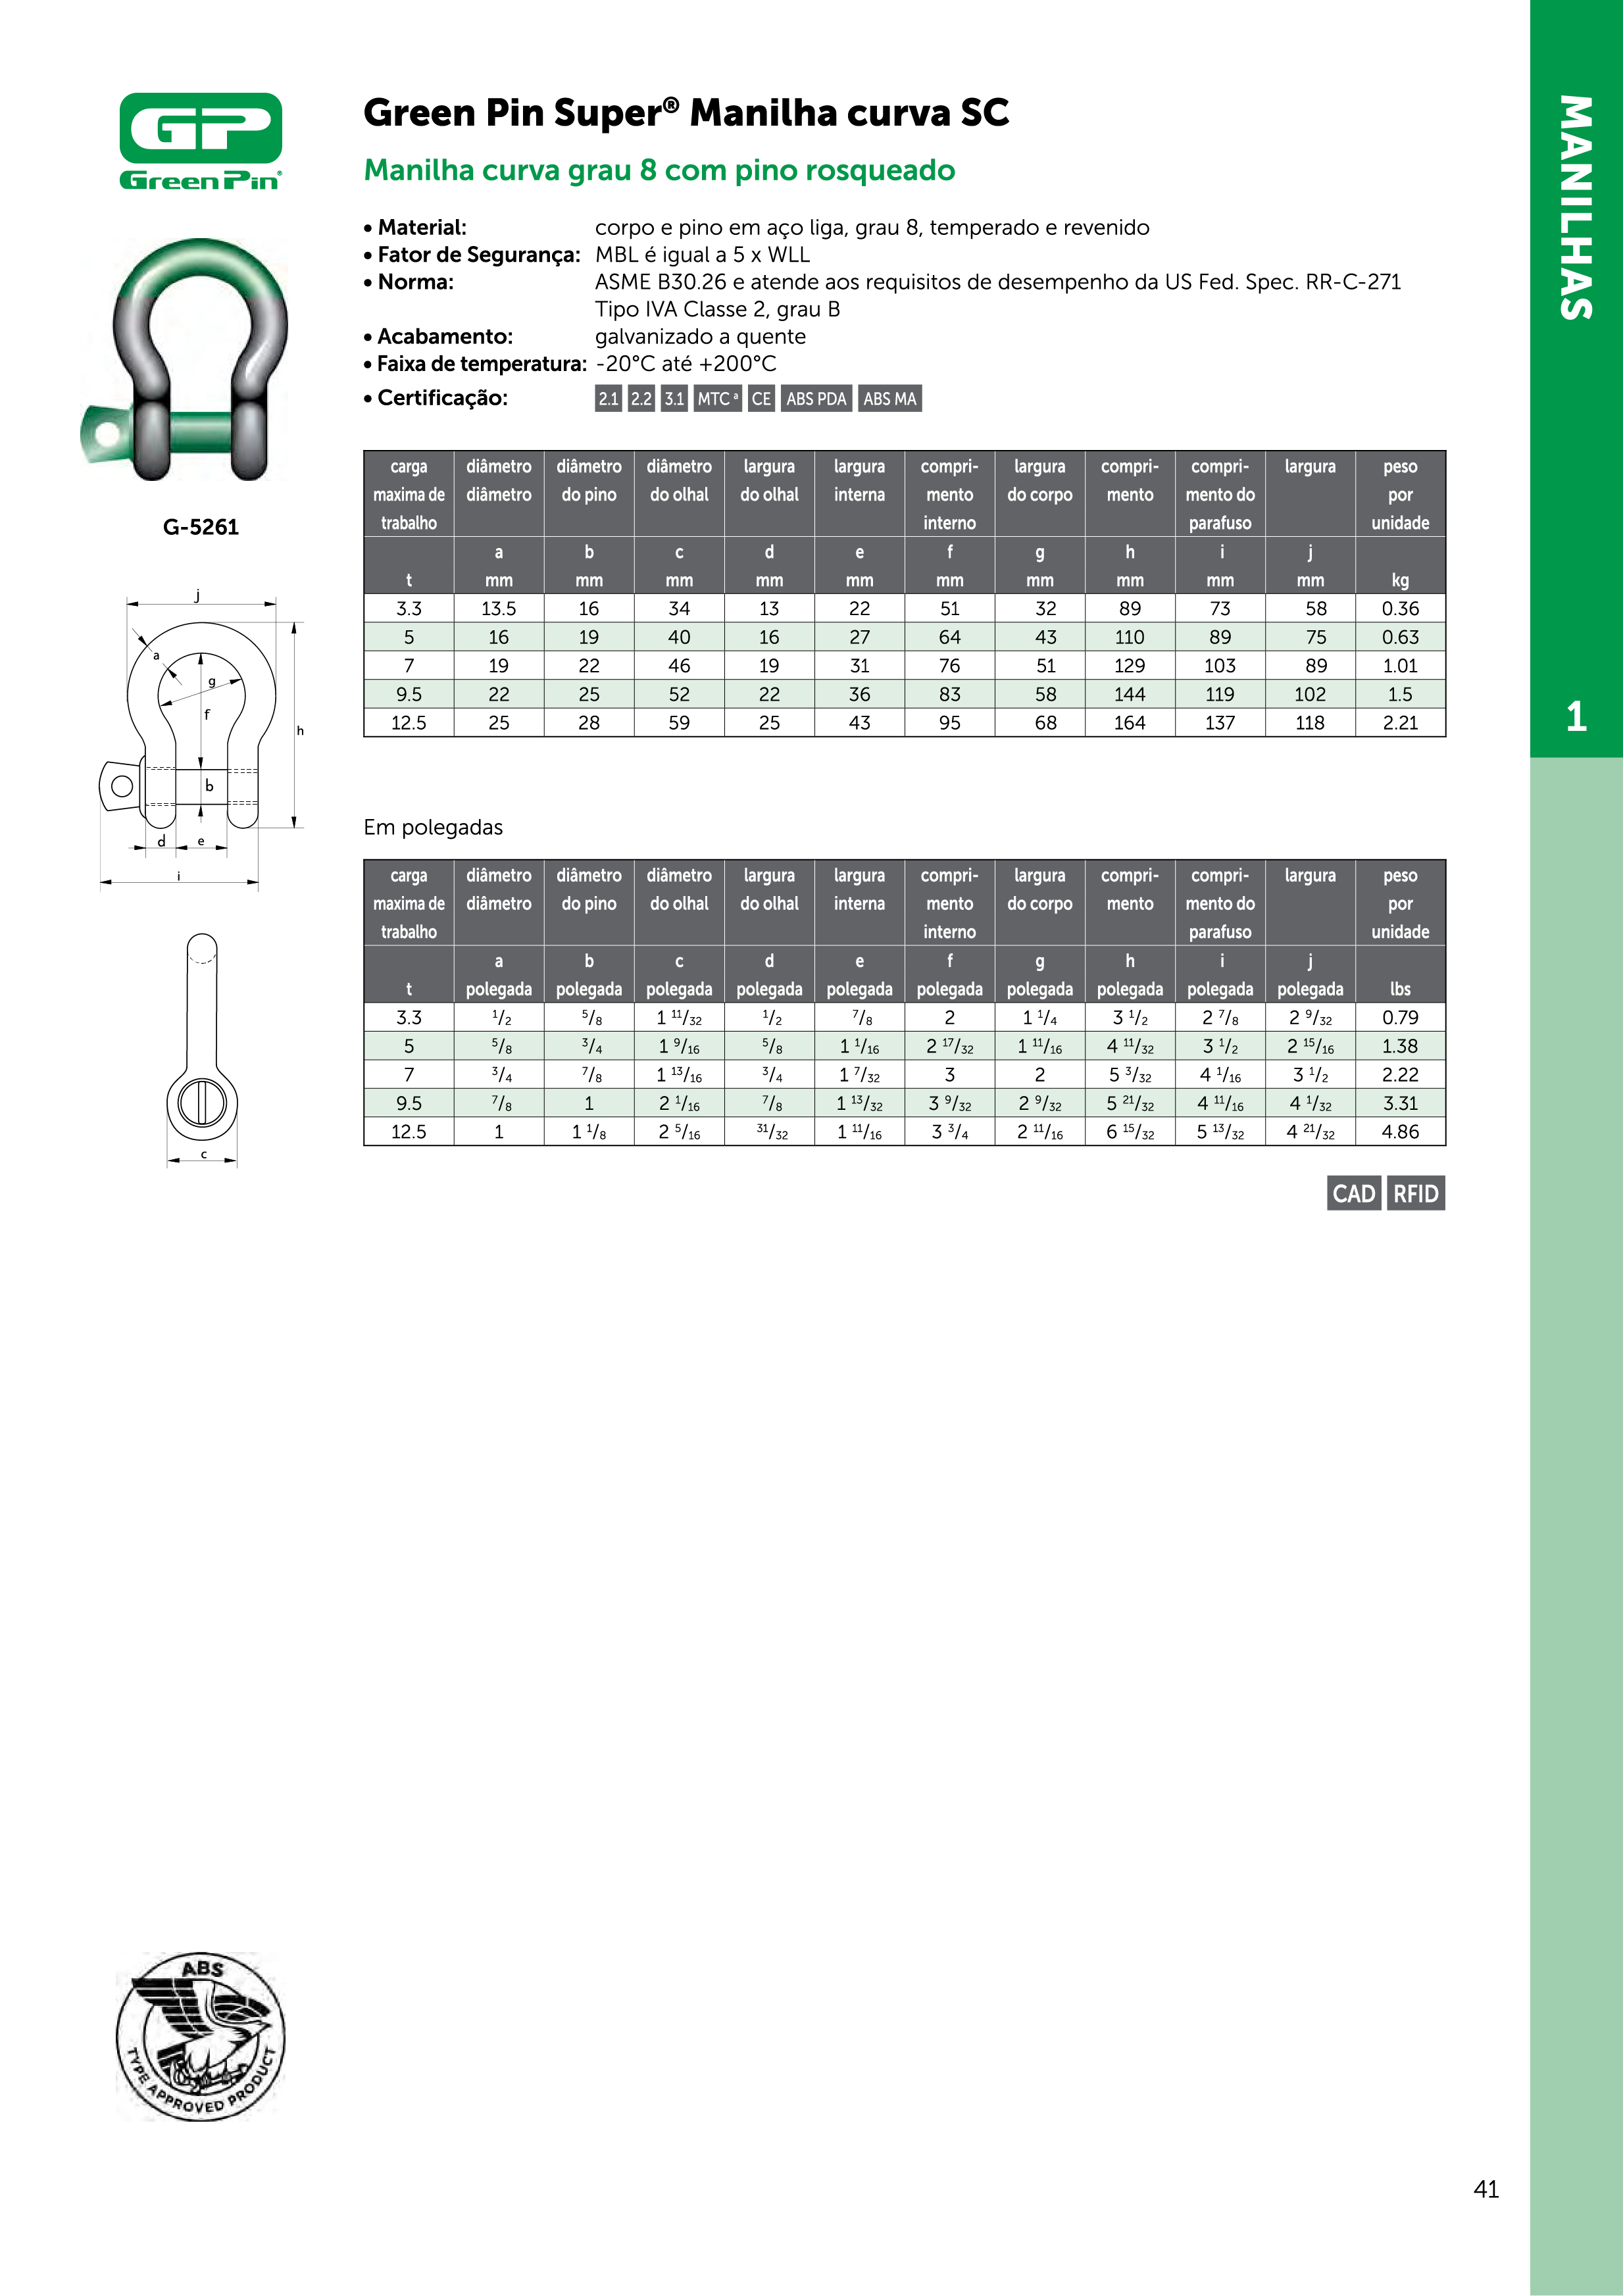
\includegraphics[width=0.85\linewidth, trim = 0 0 0 0, clip]{Figuras/Green Pin Super Manilha curva SC folha.png}\\
    \hspace{1.5cm}\raggedright \fontsize{10}{12}\selectfont{Fonte: \textcite{GreenPin}.}
    \label{catalogomanilha}
\end{figure}



%\chapter{Norma ASME B30.26.}
%\label{anexoC}

%\chapter{Norma ASME B30.26.}
%\label{anexoD}
 %    (opcional)

% \printindex %                        (opcional)

\end{document}